\chapter{Words as Trigger Points in Social Media Discussions}
\label{ch:triggers}
In the previous chapters, we examined how negativity in political dialogue can amplify engagement (\autoref{ch:political}) and how misinformation spreaders differ from users who share content from trusted sources (\autoref{ch:spreaders}). In this chapter, we shift focus to the concept of trigger points in online discussions, exploring how specific words or topics can provoke strong emotional responses and escalate polarisation.

Trigger points originate in qualitative research on political polarisation, where they were shown to capture moments when individuals felt that their understanding of what is fair, normal, or appropriate in society was challenged \citep{mau2023triggerpunkte}. In such contexts, particular words or themes sparked strong negative emotions and conflictual reactions. Extending this concept to computational research, we investigate whether similar dynamics emerge in large-scale online debates.

In this chapter, we analyse more than 100 million Reddit comments posted between 2020 and 2022 across subreddits related to UK politics, focusing on a set of words identified as political trigger points. Using transformer-based models adapted for social media, we measure sentiment and emotion, as well as the prevalence of hate speech through the classifier introduced in \Autoref{ch:hate-speech}. This enables us to capture how discussions evolve when these words appear.

Our findings show that trigger words are associated with heightened engagement and increased levels of animosity, reflected in more negative, hateful, and controversial comments. By introducing trigger points into computational studies of online communication, this chapter contributes to research on affective polarisation, online deliberation, and the dynamics of political discourse in digital environments.


\section{Introduction}
Online debates may suddenly escalate, and users intensely engage in emotional and confrontational deliberations. While these turning points are difficult to model and predict, they are essential moments in online communication. They mark the moment when a discussion is likely to get off the rails, and social media users stop debating with one another and instead debate against one another. Our study introduces trigger points as a useful concept to understand why and when social media users engage in such behaviour.

Trigger points, introduced by \citet{mau2023triggerpunkte}, are rooted in theories of affective political identity and relate to deeply lying beliefs about moral expectations and social dispositions. They open the door to modelling social media user engagement more effectively and studying the conditions and causal mechanisms that lead to adverse reactions, hate speech, and abusive language in online debates.

\begin{figure}
    \centering
    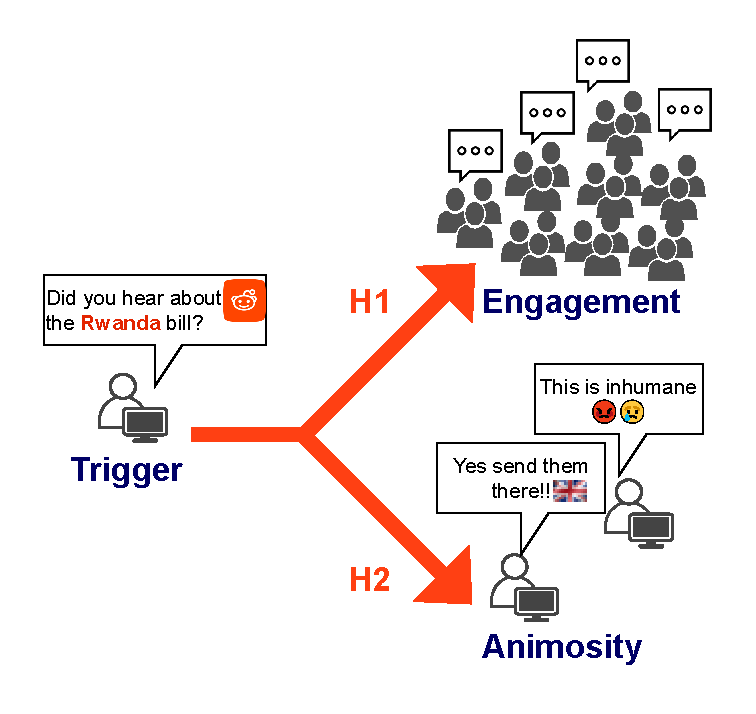
\includegraphics[clip, trim=0.7cm 0.6cm 0.4cm 0.7cm,,width=0.38\textwidth]
    {../figures/triggers/triggerpoints_icwsm-5.pdf}
    %\includegraphics[clip, trim=0.9cm 1.5cm 0.4cm 1.3cm, scale=0.6]{../figures/triggers/triggerpoints_icwsm-4.pdf}
    \caption{Consequences of trigger points. H1 refers to hypothesis 1, i.e., trigger words cause more engagement. H2 refers to hypothesis 2, i.e., trigger words cause more animosity.}
    \label{fig:triggerpoint_consequences}
\end{figure}

Trigger points are related to how individuals perceive themselves in society. People have subjective expectations about acceptable behaviour, such as explicit knowledge of law-like rules and, more importantly, an implicit understanding of appropriate actions. These deeply rooted beliefs of what is fair and unfair constitute a moral compass fundamental to navigating the social world. People feel triggered if these normative understandings are questioned. More formally, \citet[246]{mau2023triggerpunkte} define trigger points as ``\textit{those moments that question what is acceptable against the backdrop of individuals' understanding of the social contract. Trigger points jeopardise what individuals consider the fabric of society and their own role in it.}'' 
The authors suggest that trigger points can affect individuals through four mechanisms. 
\begin{itemize}
\item \textbf{Inequality.} When expectations about equality might not be met. Either similar people are treated unequally, or, to the contrary, people who should be treated differently are treated the same. For example, social benefits might be at eye level with minimal wage earners. 
\item \textbf{Norm transgression.} It is the transgression of what is considered ``normal'' behaviour. A typical example relates to the lavish lifestyle of the privileged. 
\item \textbf{Slippery slope.} There could be a fear of society developing norms about appropriate behaviour that goes in subjectively undesired directions and the impression that the individual might not have the power to do something against it. Claims such as ``Opening the borders so that a country could be flooded with immigrants'' is an example. 
\item \textbf{Behavioural demands.} When society may be perceived as demanding unreasonable behaviour. The role of pronouns is a point in case where the generic masculine pronouns ``he/him'' might trigger some, and the neutral pronoun ``they/them'' might trigger others.
\end{itemize}
% Reacting to triggerpoints
Going against deeply held beliefs about individuals and their societal role causes discomfort. People respond to such triggers in an affective behavioural mode, increasing a debate's intensity and emotionality. %\citep{mau2023triggerpunkte}. 

In the social media context, we expect that this has two direct consequences (Figure~\ref{fig:triggerpoint_consequences}). Trigger points lead to:
\begin{itemize}
    \item \textbf{Hypothesis 1:} more user engagement, which leads to more messages or comments.
    \item \textbf{Hypothesis 2:} higher levels of animosity, which causes polarisation, negativity, anger, and hate.
\end{itemize}

Our study seeks to establish the concept of trigger points in online communication. The research design and case selection closely follow this logic and examine whether and how individual words can act as trigger points in online debates. To this end, we conduct a large-scale case study and select five words that are \emph{ex-ante} likely to work as trigger points in the context of UK politics. Specifically, we look into the words \textit{Rwanda, Brexit, NHS, Vaccine, Feminism}. Collecting $>$100 million related Reddit comments, we use text analytics and NLP methods to understand whether these words lead to potentially negative, emotional, and harmful responses. The analysis builds upon a systematic comparison between a treatment and control group in three different scenarios:
\begin{enumerate}
    \item \textit{Space}: specific subreddits where the selected words trigger users.
    \item \textit{Contextual}: words that appear in a similar context to the target words but without the triggering component.
    \item \textit{Time:} periods identified as relevant for each specific trigger word. 
\end{enumerate}

We find that the trigger words cause higher engagement and more animosity, measured as an increase in a thread's controversiality, negative sentiment, anger, and hate speech.

\section{Related Work}
Existing work studies how particular political words or phrases lead to more engagement \cite{Brady17, Hameleeres21} and posts with more emotion and animosity \cite{friedman2004positive, Martin_Huck_Williams_Hull_Hull_2021, Schroth2005stones, Rho20} in various online settings. However, they lack a joint conceptual and theoretical framework\textemdash something we aim to provide.

Trigger points are fundamental to understanding polarisation and division in online discussions. Given that they are at the root of different conflictive behaviours later on, they help understand the causes of disagreements in online conversations \cite{de-kock-vlachos-2021-beg2} and their escalation \cite{de-kock-vlachos-2022-disagree,van-der-meer-etal-2023-differences} triggering explicit and implicit \textit{ad hominem} attacks, hate speech, abusive or offensive language on social media \cite{Talat2016HatefulSO, davidson2017automated,basile2019semeval,ousidhoum-etal-2019-multilingual,sap-etal-2019-social2, elsherief-etal-2021-latent2, ocampo-etal-2023-depth}.


Similarly, considering the broad array of harmful online behaviours, the wide range of elements they involve, and how they can be included in social media data \cite{olteanu2019social}, \citet{blodgett-etal-2020-language2} report a missing paradigm that helps assess the initial causes without mainly focusing on the performance of the detection model. Studying trigger points helps track the origins of bias, assess whether a social media post can lead to toxic comments \cite{dahiya2021would}, and how language affects polarisation on social media \cite{Karjus2024}. It lays the groundwork for understanding how polarised rhetoric may emerge and lead to intergroup conflict \cite{Almog22}.


Related to trigger points are dog-whistles\textemdash coded expressions that carry two meanings: a seemingly harmless one, and another one with a hidden hateful or provocative connotation that only insiders can decipher \cite{breitholtz-cooper-2021-dogwhistles2}. In social sciences, the concept of dog whistle has its roots in the study of racial politics in the United States, leading politicians to develop more subtle ways of appealing to racial prejudices \cite{lopez2013dog} and has evolved to encompass a broader range of phenomena, ranging from perpetuated systemic racism \cite{Filimon03032024}, to more broadly communication strategies of political ambiguity in identity politics\cite{Tolvanen24}, such as religion \cite{perry2023mating} or immigration \cite{filimon2016dog}. Trigger points are similar in their equivocality and potential to evoke emotional responses. Conversely, using a dog whistle is conscious, but there is typically no intent when relying on trigger points. Moreover, while dog whistles are rhetorical devices to hide the real intention from some and create a rally-around-the-flag effect, trigger points are not hidden communication and incite a strong sense of otherness towards those covered by the trigger. 

Research on the automation of identifying affective triggers in online discussions remains limited. For instance, \citet{almerekhi2022provoke} developed a framework to identify triggers for toxic behaviour within Reddit discussions. Similar work typically uses a restricted set of lexical features, primarily sentiment analysis, and often examines the level of engagement some topics may generate \cite{aldous2023really}. Others, such as \citet{beel2022linguistic}, explicitly investigate highly controversial topics like abortion, climate change, and gun control, attempting to predict contentiousness within discussions, often heavily relying on Reddit comment upvote ratios as a proxy for contentiousness.
Finally, some studies focus on online conversational tensions by predicting conversational derailment, considering the overall progression of a conversation rather than specific terms as causes \cite{zhang2018conversations,hessel2019something}.


\section{Methodology}
To empirically demonstrate that individual words can trigger online debates, we look into most likely cases in the context of UK politics. Based on a curated set of likely candidate words for the political context in the UK (see Section \ref{subsec:term_selection}), we test whether individual words can trigger the reactions outlined in the two hypotheses, i.e., (1)\ more engagement and (2)\ animosity. Our goal is to report behavioural mechanisms similar to those observed by \citet{mau2023triggerpunkte} when conducting interviews to analyse the perceived polarisation. If we could \textbf{not} find these effects in these intuitive cases, we would falsify the theory for online contexts.


\subsection{Term selection}\label{subsec:term_selection}
We selected \textit{National Health Service (NHS)}, \textit{Brexit}, \textit{Rwanda}, \textit{Vaccine}, and \textit{Feminist/Feminism}. These terms are associated with high-profile public debates, policy changes, and social movements in the UK. Hence, they typically provoke significant public engagement and emotional responses. We expect them to cause the intended reactions in British social media users. Table~\ref{tab:trigger_word_choices} indicates mechanisms through which the terms may trigger individuals. 


\begin{table}[]
\centering
\scalebox{0.9}{ % adjust the scale factor (0.9 = 90%)
\begin{tabular}{lccccc}
%\toprule
                    & \textbf{Rwanda} & \textbf{Brexit} & \textbf{NHS} & \textbf{Vaccine} & \textbf{Feminism} \\ \hline
\textbf{Inequality}          &  \checkmark     &    \checkmark   &  \checkmark  &    \checkmark    &           \\ \midrule
\textbf{Norm transgression}  &        &    \checkmark   &     &         &    \checkmark      \\ \midrule
\textbf{Slippery Slope}      &  \checkmark     &    \checkmark   &     &    \checkmark    &    \checkmark      \\ \midrule
\textbf{Behavioural Demands} &        &        &     &    \checkmark    &    \checkmark      \\ \bottomrule

\end{tabular}}
\caption{Trigger words and their respective trigger mechanisms (described in the introduction).}
\label{tab:trigger_word_choices}
\end{table}

\paragraph{Rwanda.} 
Until late 2021, Rwanda was just the name of any other African country. However, in early 2022, the term's meaning became emblematic of how the British government suggested handling asylum seekers, and the home secretary struck a deal with Rwanda: the \textit{Migration and Economic Development Partnership}.\footnote{https://www.gov.uk/government/publications/uk-rwanda-treaty-provision-of-an-asylum-partnership/uk-rwanda-treaty-provision-of-an-asylum-partnership-accessible} With this agreement, \textit{Rwanda} became a trigger word for discussions on immigration policy in the UK from 2022 onwards, particularly related to ``unfair favours towards migrants and unregulated immigration'' \cite{economist2023rwandan}.

\paragraph{Brexit.} The UK's departure from the European Union has been controversial since its inception. The division among the population was already evident during the tightly contested 2016 referendum\cite{ARNORSSON2018301}. Additionally, misinformation and disinformation have intensified these debates \cite{holler2021human,bruno2022brexit}. Here, considerations about treating EU migrants differently than the national population (inequality), norm transgressions of ``criminal'' migrants, particularly from Eastern Europe, or opening the gate to ``unlimited'' immigration make \textit{Brexit} a potential trigger word for analysis.

\paragraph{NHS.} Due to financial austerity measures, the UK government was accused of reducing its budget and neglecting the healthcare system \cite{guardian2022nhsbacklog, independent2024nhs}. Public opinion is divided, with some supporting that the NHS receives adequate funding, while others believe it wastes resources or that its services are in decline \cite{gershlick2015public}. This trigger word is related to going against considerations about unequal treatment (i.e., inequality as shown in Table \ref{tab:trigger_word_choices}).


\paragraph{Vaccine.} Public vaccination programs, particularly those against COVID-19, have caused significant debate in recent years. %Even after their widespread roll-out, discussions over their effectiveness and safety are ongoing. 
Post-roll-out, debates have shifted to focus on issues such as the fairness of vaccine distribution and unreasonable demands for vaccination \cite{nichol2021ethics}. Moreover, the proliferation of misinformation and conspiracy theories has further fuelled public division \cite{hayawi2022anti, garett2021online}, particularly in social media, making \textit{Vaccine} an ideal trigger word for our study.

\paragraph{Feminism.} Misogyny can be observed on social media, where anonymity often allows users to express offensive and hateful sentiments \cite{barker2019online}. Some social media influencers have built a large audience by sharing and promoting harmful content against women. This has led to the formation of online echo chambers \cite{farrell2019exploring} where such views are amplified and propagated. Our research includes \textit{Feminism} as a trigger word based on mechanisms related to norm transgressions, fears of a slippery slope, and unreasonable behavioural demands. 


\begin{table}[]
\centering
\scalebox{0.9}{ % adjust the scale factor (0.9 = 90%)
\begin{tabular}{ll}
\toprule
\textbf{Keyword} & \multicolumn{1}{c}{\textbf{Subreddits}} \\ \hline
\textbf{Feminism} & \begin{tabular}[c]{@{}l@{}}AskMen, MensRights, \\ antifeminists, AndrewTateTalk\end{tabular} \\ \hline
\textbf{Brexit} & \begin{tabular}[c]{@{}l@{}}neoliberal, brexit, ireland, unitedkingdom, \\ The\_Donald, ukpolitics, tories, \end{tabular} \\ \hline
\textbf{NHS} & \begin{tabular}[c]{@{}l@{}}neoliberal, CoronavirusUK, unitedkingdom,\\ ukpolitics, tories, labourUK\end{tabular} \\ \hline
\textbf{Rwanda} & \begin{tabular}[c]{@{}l@{}} neoliberal, tories, labourUK, currenteventsuk\\ ukpolitics, uknews, unitedkingdom \end{tabular} \\ \hline
\textbf{Vaccine} & \begin{tabular}[c]{@{}l@{}}conspiracy, neoliberal, unpopularopinion, \\ antifascistsofreddit, coronavirusuncensored, \\  CoronavirusUK, Coronavirus, wuhan\_flu  \end{tabular} \\ \hline
\end{tabular}}
\caption{Subreddits selected for each trigger word. }
\label{tab:keywords_subreddits}
\end{table}


\begin{table}[ht]
\centering
\resizebox{\textwidth}{!}{
\begin{tabular}{lcccc|cccc|cccc|cccc|ccrr}
\toprule
 & \multicolumn{4}{c|}{\textbf{Feminist}} & \multicolumn{4}{c|}{\textbf{Rwanda}} & \multicolumn{4}{c|}{\textbf{Brexit}} & \multicolumn{4}{c|}{\textbf{NHS}} & \multicolumn{4}{c}{\textbf{Vaccine}} \\
 & \textbf{Be} & \textbf{Af} & \textbf{DiD} & \textbf{CI} & \textbf{Be} & \textbf{Af} & \textbf{DiD} & \textbf{CI} & \textbf{Be} & \textbf{Af} & \textbf{DiD} & \textbf{CI} & \textbf{Be} & \textbf{Af} & \textbf{DiD} & \textbf{CI} & \textbf{Be} & \textbf{Af} & \multicolumn{1}{c}{\textbf{DiD}} & \multicolumn{1}{c}{\textbf{CI}} \\ \hline
\textbf{\begin{tabular}[l]{@{}l@{}}Treatment\\ Only\end{tabular} } & 47 & 53 & \multicolumn{2}{c|}{} & 45 & 55 & \multicolumn{2}{c|}{} & 46 & 54 & \multicolumn{2}{c|}{} & 46 & 54 & \multicolumn{2}{c|}{} & 47 & 53 & \multicolumn{1}{c}{} & \multicolumn{1}{c}{} \\ \hline
\textbf{Space} & 49 & 51 & \textbf{4.1} & (3.8, 4.5) & 50 & 50 & \textbf{9.7} & (8.2, 11.3) & 49 & 51 & \textbf{6.3} & (6.1, 6.6) & 49 & 51 & \textbf{6.1} & (5.7, 6.4) & 49 & 51 & \textbf{4.1} & (3.5, 3.9) \\
\textbf{Contextual} & 48 & 52 & \textbf{4.6} & (3.9, 5.2) & 50 & 50 & \textbf{9.8} & (6.6, 14.9) & 47 & 53 & \textbf{3.2} & (2.6, 3.7) & 53 & 47 & \textbf{13.4} & (8.7, 18.1) & 49 & 51 & \textbf{5.0} & (3.1, 6.9) \\
\textbf{Temporal} & \multicolumn{4}{c|}{-} & 49 & 51 & \textbf{7.2} & (2.9, 11.6) & \multicolumn{4}{c|}{-} & \multicolumn{4}{c|}{-} & 50 & 50 & \textbf{5.9} & (4.1, 7.6) \\ \bottomrule
\end{tabular}}
\caption{Percentage of comments per thread before (Be) and after (Af) each trigger appearance (Hypothesis 1). Difference-in-Difference (DiD) and 95\% confidence interval (CI) included for the Control, Space and Contextual, comparisons. Bold scores indicate statistically significant results. Detailed distribution of comments can be seen in Appendix \ref{sec:appendix_counts}, see Figure \ref{fig:absolute_counts_overall}.}
\label{tab:trigger-counts}
\end{table}

\subsection{Data collection}
\label{sec:data_collection}
Our study uses data from Reddit comments in English, collected via the Pushshift API \cite{baumgartner2020pushshift}. We searched for exact matches of specific keywords in comments from 2019 to 2022 and then collected the entire discussion thread for each extracted comment.\footnote{When extracting comments for the term \textit{woman}, we capped the maximum number of comments at 20 million due to the large volume.} 
We excluded comments in languages other than English, identified as such using a fastText-based language identifier \cite{bojanowski2017enriching}. Comments marked as ``[deleted]'' by the API were also removed. Following this, only threads that contained comments before and after the appearance of the target keywords were retained, as it is crucial to analyse the potential differences before and after the appearance of a given trigger point. 

As a final filtering step, we limited our analysis to comments 30 minutes before and 30 minutes after the first mention of the triggering word. Previous research has shown that Reddit comments typically receive the majority of interactions within a short window after the comment is created \cite{thukral2018analyzing}. Moreover, early responses are often important in shaping the direction of the conversation \cite{singer2016evidence,horne2017identifying}. Considering the fast-paced nature of Reddit, the 30-minute window filters out unrelated responses and ensures the focus of our analysis remains on the most relevant data\footnote{Table \ref{tab:trigger_counts} in Appendix \ref{sec:appendix_counts} shows the total number of comments, threads, and comments collected for each trigger word and the period they were gathered.}.

\subsection{Research design}
We identify the causal effect of trigger points with the difference-in-difference estimator (DiD), which systematically compares a treatment with a control group \citep{angrist2009mostly, Card1994}. It calculates the causal effect of an intervention as the difference before and after the intervention in the treatment group minus the difference before and after the intervention in the control group. In our context, we expect users in the treatment group to be highly likely to be triggered by the respective terms and those in the control group to be much less triggered by the respective words. There should be a more substantive behavioural change for the treatment group than for the control group. 

\subsubsection{Control groups}
We systematically compare treatment and control groups along three different dimensions.\footnote{Identifying the causal effect in three completely unrelated comparisons helps address concerns about eventual endogeneity.}

\paragraph{1. Space}
Discussions on Reddit are structured in different fora, also called subreddits. Aiming to investigate the effects a trigger word might have on specific subsets of users, we define the treatment group as a set of popular subreddits related to the trigger word (Table \ref{tab:keywords_subreddits}). We compare them with discussions in a control group, i.e., the rest of Reddit with many non-domain specific subreddits. 

\paragraph{2. Contextual} 
We also compare trigger words with terms that appear in a similar context, but that does not go against the more profound underlying transgressions responsible for trigger responses in similar contexts. To members of the subreddits in Table~\ref{tab:keywords_subreddits}, using an explicit trigger word or its more harmless control term should make a real difference. We define related control group words and contrast \textit{woman} to \textit{Feminism/Feminist}, \textit{Red Cross} to \textit{NHS}, \textit{EU/European Union} to \textit{Brexit}, \textit{surgery} to \textit{vaccine}, and names of Rwanda's neighbouring countries\footnote{Burundi, Tanzania, Congo, Democratic Republic of Congo, Uganda, Kenya, and Zambia.} to \textit{Rwanda}. Treatment and control groups are from the same subreddits in the same year.

\paragraph{3. Temporal}
In the third experiment, we use the fact that two of our terms\textemdash \textit{Vaccine} and \textit{Rwanda}\textemdash only became explicit trigger words at specific points in time. For ``Rwanda'', we compare discussions in subreddits likely to spark reactions in 2020 to discussions in 2022. For \textit{Vaccine} we compare threads from 2019 (before the COVID-19 pandemic) to 2022's (post COVID-19 pandemic). Again, we expect that users from the subreddits in Table~\ref{tab:keywords_subreddits} are triggered by those only in 2022 but not in the respective earlier years. Treatment and control groups share the same subreddits but are from different years.


\subsubsection{Statistical analysis}
We estimate the trigger words' treatment effect in 60 separate experiments\textemdash 12 experiments for H1 (Table~\ref{tab:trigger-counts}) and 48 experiments for H2 (Table~\ref{tab:trigger-results}). For each experiment, we prepare the data in the same way. The treatment is the first mention of a trigger word in a discussion thread, i.e., there is only one well-defined treatment per thread. 
To test H1, we count the number of comments for each discussion thread 30 minutes before and 30 minutes after the treatment in the treatment group and the placebo treatment in the control group. We then calculate the share of comments before and after the intervention. For example, if there are 8 comments during the 30 minutes before the trigger word and 12 comments during the 30 minutes after the trigger word, we normalize the data of this discussion thread to 40\% before intervention and 60\% after intervention. For experiments with H2, we count the number of comments expressing animosity in a thread and then normalize the data as a share of animosity per thread before and after the trigger word.

We estimate the causal effect in an OLS-regression framework. More specifically, we specify the DiD with the two-way fixed effects estimator \cite{angrist2009mostly}:
\[
\text{proportion} \sim \text{trigger\_dummy} + \text{treatment\_dummy} + \text{interaction}
\] where \textit{proportion} is the per-thread-normalised target feature and the interaction term is given by
\[
\text{interaction} = \text{trigger\_dummy} \times \text{treatment\_dummy}.
\]

Since the DiD estimator subtracts the difference before and after intervention in the control from the equivalent in the treatment group, no further control variables are necessary\textemdash if the parallel trends assumption holds \cite{roth2023s}. It requires that in the absence of treatment, the difference between the outcomes of the treated and control groups would follow the same trajectory over time. We investigate the plausibility of the assumption in section \ref{sec:parallel_trends}.

\subsection{Features} \label{sec:features}
We rely on several features to examine our initial hypotheses and study the impact of trigger words in online discussions. We use comment counts for the first hypothesis (H1) about user engagement. The second hypothesis (H2) requires a measure of animosity. To identify relevant features that can operationalize animosity, we build on various language models that follow the RoBERTa architecture \cite{ROBERTA} and are trained in social media corpora, specifically \textit{X} (Twitter). Even though comments on Reddit tend to be longer than on \textit{X}, the posts on both platforms share many similarities, e.g., the use of slang, emojis, or unstructured text. Hence, we expect the trained models to perform well in either context \cite{priya2019should}. 
 
\subsubsection{User engagement (Hypothesis 1)}
Our first hypothesis suggests that trigger words lead to higher user engagement. We rely on the number of comments to investigate this and expect an uptick in message frequency after the trigger words are mentioned for the first time in a thread.

\subsubsection{Animosity (Hypothesis 2)}
Hypothesis 2 suggests that trigger words cause more animosity in a debate. We operationalize this with controversial comments, negative sentiment, anger, and different forms of hate speech.

\paragraph{Controversiality} We examine whether a comment is controversial using the Reddit controversiality feature. Reddit offers a measure that identifies a comment as controversial if it receives similar amounts of upvotes and downvotes. This metric is based on the users' approval, so care must be taken when considering already controversial subreddits. We expect trigger words to cause more controversiality.


\begin{figure}[t!]
    \centering
    \scalebox{1}{
    \resizebox{\columnwidth}{!}{
    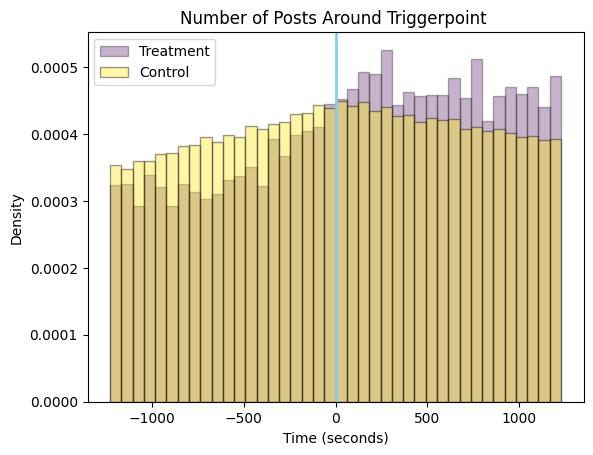
\includegraphics{../figures/triggers/counts/counts_space/counts_space_rwanda.png}
    }}
    \caption{Distribution of comments in the treatment and control groups (space) for  the trigger word \textit{Rwanda}.}
    \label{fig:counts_space_rwanda}
\end{figure}


\paragraph{Sentiment analysis} For sentiment analysis, we use \textit{twitter-roberta-base-sentiment-latest} \cite{loureiro-etal-2022-timelms} which identifies a comment as \textit{negative, neutral, or positive}. This model has been fine-tuned for sentiment analysis using the SemEval 2017 Sentiment Analysis dataset \cite{rosenthal2019semeval}. As we expect trigger words to cause more negative sentiments, we use sentiment analysis to investigate this, similarly to work using it to gain insights into how controversial topics such as vaccination \cite{melton2021public}, politics \cite{guimaraes2019analyzing}, and gender biases \cite{marjanovic2022quantifying} are discussed online.


\paragraph{Negative emotions} 
We leverage \textit{twitter-roberta-base-emotion-multilabel-latest} \cite{camacho2022tweetnlp} to assign one or more emotions to each tweet. This model is trained on the Semeval 2018 Affect in Tweets task \cite{mohammad2018semeval}, covering 11 different emotions.\footnote{Detailed list of emotions can be found in Appendix \ref{sec:triggers-emotion-list}}) For our analysis, we focus on anger specifically, and we expect to observe more anger after a trigger word.


%% DIMOS move here
\begin{figure}
    \centering
    \resizebox{\columnwidth}{!}{
    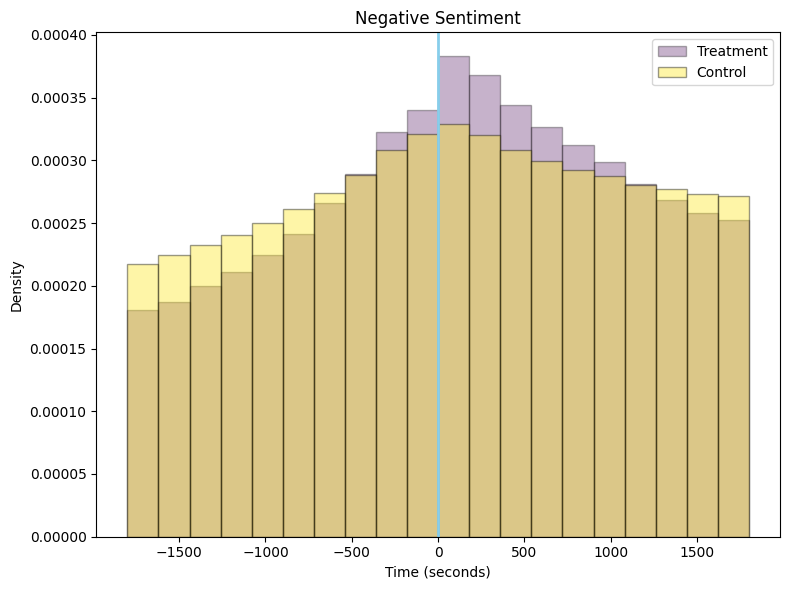
\includegraphics{../figures/triggers/sentiment/space/vaccine.png}
    }
    \caption{Distribution of negatively charged comments for the treatment and control (space) groups of \textit{Vaccine} as a trigger word.}
    \label{fig:sentiment_space_vaccine}
\end{figure}

\paragraph{Hate speech} Finally, we use the \textit{twitter-roberta-base-hate-multi-class} model \cite{antypas2023robust} to detect hate speech. It is trained on a combination of 13 different hate speech Twitter datasets and can predict hate towards seven target groups.\footnote{Detailed list of categories can be found in Appendix \ref{sec:triggers-hate-list} }) The inclusion of hate speech detection as a feature is motivated by previous research revealing hateful trends in topics such as politics \cite{rieger2021assessing}, women's rights \cite{farrell2019exploring}, and health issues \cite{walter2022vaccine}. Considering the connotations of some of the triggers, we specifically focus on sexism for \textit{Feminism/Feminist} and racism for \textit{Rwanda}. For \textit{NHS}, \textit{Brexit} and \textit{Vaccine} we consider all hateful comments jointly.

\subsection{Validation of Annotation Model}

The primary aim of our research is %not to develop or employ the most sophisticated classifiers, but rather 
to use simple and computationally efficient models that reliably extract signals relevant to our hypotheses. To confirm the validity and robustness of our findings, we implemented an additional validation procedure to ensure consistency across the classifiers employed in our analysis.

We sampled 100 Reddit comments from our data collection, with 20 comments selected from the subreddits associated with each trigger point (Table \ref{tab:keywords_subreddits}). %Given the relative infrequency of hate speech, we ensured that each trigger included four comments previously classified as hate speech by our original model (20\% of the dataset). 
The collected comments were independently annotated by three experienced NLP and CSS researchers for sentiment, emotion, and the presence of hate speech.\footnote{We include the annotation guidelines in Appendix \ref{sec:appendix_guidelines}.} Each comment was assigned a label based on the majority vote, while disagreements were resolved through discussion. When considering the difficulty of the annotation task, the annotations present above-average agreement scores for sentiment and hate speech, with Fleiss' $\kappa$ scores of 0.52 and 0.56, respectively. For the multi-label emotion annotation task, where annotators had to choose from a set of 12 labels,the Krippendorff’s alpha score \cite{krippendorff2011computing} reached 0.24, which is in line with other similar multi-label tasks with a high number of labels \cite{mohammad2018semeval,antypas2022twitter,ousidhoum-etal-2019-multilingual}.

We fine-tune the base version of BERT-cased, XLNet, and RoBERTa for sentiment analysis, emotion recognition, and hate speech detection on the same datasets as the models we used for our experiments, as explained in Section \ref{sec:features} \cite{rosenthal2017semeval,mohammad2018semeval,antypas2023robust} to ensure fairness.
%\dimos{Five different models, BERT-cased and XLNET, base and large variations, along with the vanilla RoBERTa-base, which the models we utilise are based on, are fine-tuned for sentiment analysis, emotion classification, and hate speech detection using the same datasets with the models used for our experiment
We further compare our results to those of five pre-trained models publicly available on HuggingFace. Specifically, two sentiment classifiers trained on Reddit data\footnote{ reddit-dBERT: \url{https://huggingface.co/akshataupadhye/finetuning-sentiment-model-reddit-data}, reddit-XLNET: \url{https://huggingface.co/minh21/XLNet-Reddit-Sentiment-Analysis} }, hateBERT \cite{caselli-etal-2021-hatebert2} and one emotion classifier\footnote{BERT-emotion: https://huggingface.co/ayoubkirouane/BERT-Emotions-Classifier}. All models are evaluated in the aforementioned manually labelled dataset.

Table \ref{tab:models_evaluation} presents the average micro F1-scores achieved by the models across each task. We opted for the micro F1-score as it provides a more realistic representation of the results, given the limited sample and heavily imbalanced nature of our dataset.\footnote{Detailed dataset distribution is available in Appendix \ref{sec:validation}} The Twitter-RoBERTa models achieved the highest scores on all tasks.%, scoring 76\%, 50\%, respectively. 
These scores are matched by XLNet-base for sentiment analysis and XLNet for emotion detection, and the fine-tuned models RoBERTa and XLNet for hate speech detection. %For hate speech detection, the fine-tuned XLNet, BERT, along with Twitter-RoBERTa models demonstrated the highest performance with a score of 88\%. %The performance gap can be attributed to the significant class imbalance (e.g. the small number of hateful entries, with only 10 instances present in the test set). 
Overall, the tested models performed comparably well, except for two off-the-shelf sentiment classifiers that achieved scores below 50\%. %These findings serve as a validation of our model selection, confirming robust performance despite using models trained initially for Twitter and not Reddit. %and supporting the integrity of our analysis.

\begin{table}[h]
\centering
\begin{tabular}{l|c|c|c}
\hline
\textbf{}    & \textbf{Sentiment} & \textbf{Emotion} & \textbf{Hate} \\ \hline
t-RoBERTa    & \textbf{0.76}      & \textbf{0.50}    & \textbf{0.88}          \\
RoBERTa    & 0.75               & 0.47             & \textbf{0.88}          \\
XLNet      & \textbf{0.76}      & 0.45             & \textbf{0.88}         \\
BERT       & 0.74               & 0.40             & 0.85          \\
reddit-dBERT & 0.45               & -                & -             \\
reddit-XLNet & 0.31               & -                & -             \\
BERT-emotion & -                  & 0.45             & -             \\
hateBERT     & -                  & -                & 0.80          \\ 
Random     &  0.30                  & 0.20                & 0.07         \\ \hline
\end{tabular}
\caption{Average micro-F1 scores of the models tested for the sentiment analysis, emotion, and hate speech detection tasks. \textit{Random} indicates a naive baseline that randomly selects labels.}
\label{tab:models_evaluation}
\end{table}

\section{Results}
\subsection{User engagement (Hypothesis 1)}
\begin{table}[t!]
\centering
\captionsetup[subtable]{justification=centering}
\setlength{\tabcolsep}{4pt}        % tighter columns
\renewcommand{\arraystretch}{1.1}  % a bit of breathing room

\begin{subtable}[t]{0.49\textwidth}
\centering\small
\begin{tabular}{cc|ccc}
\textbf{Trig.} & \textbf{Set.} & \textbf{Feature} & \textbf{DiD} & \textbf{CI} \\ \hline

\multirow{8}{*}{\rotatebox{90}{Brexit}} & \multirow{4}{*}{\rotatebox{90}{Space}} & Contr & \textbf{1.0} & (0.8, 1.3) \\
 &  & N.Sent & \textbf{3.3} & (3.0, 3.5) \\
 &  & Anger & \textbf{2.7} & (2.4, 3.0) \\
 &  & Hate & -0.1 & (-0.5, 0.4) \\ \cline{2-5} 
 & \multirow{4}{*}{\rotatebox{90}{Context.}} & Contr & \textbf{1.4} & (0.7, 2.1) \\
 &  & N.Sent & \textbf{2.6} & (2.0, 3.1) \\
 &  & Anger & \textbf{3.8} & (2.1, 5.5) \\
 &  & Hate & -0.5 & (-1.9, 0.9) \\ \hline
\multirow{8}{*}{\rotatebox{90}{Feminist}} & \multirow{4}{*}{\rotatebox{90}{Space}} & Contr & 0.3 & (-0.2, 0.8) \\
 &  & N.Sent & \textbf{2.6} & (2.2, 3.0) \\
 &  & Anger & \textbf{1.4} & (1.0, 1.9) \\
 &  & Sexism & \textbf{0.6} & (0.1, 1.1) \\ \cline{2-5} 
 & \multirow{4}{*}{\rotatebox{90}{Context.}} & Contr & 0.1 & (-0.8, 1.1) \\
 &  & N.Sent & \textbf{3.0} & (2.3, 3.6) \\
 &  & Anger & \textbf{1.4} & (1.0, 1.9) \\
 &  & Sexism & \textbf{1.4} & (0.5, 2.3) \\ \hline
\multirow{8}{*}{\rotatebox{90}{NHS}} & \multirow{4}{*}{\rotatebox{90}{Space}} & Contr & \textbf{1.1} & (0.7, 1.4) \\
 &  & N.Sent & \textbf{3.1} & (2.8, 3.5) \\
 &  & Anger & \textbf{2.7} & (2.3, 3.1) \\
 &  & Hate & -0.3 & (-0.9, 0.3) \\ \cline{2-5} 
 & \multirow{4}{*}{\rotatebox{90}{Context.}} & Contr & 4.5 & (-3.2, 12.2) \\
 &  & N.Sent & 3.5 & (-1.2, 8.3) \\
 &  & Anger & 4.2 & (-11.6, 20.0) \\
 &  & Hate & -1.4 & (-12.5, 9.6)
\end{tabular}
\end{subtable}\hfill
\begin{subtable}[t]{0.49\textwidth}
\centering\small
\begin{tabular}{cc|ccc}
\textbf{Trig.} & \textbf{Set.} & \textbf{Feature} & \textbf{DiD} & \textbf{CI} \\ \hline
\multirow{12}{*}{\rotatebox{90}{Rwanda}} & \multirow{4}{*}{\rotatebox{90}{Space}} & Contr & \textbf{2.3} & (0.8, 3.7) \\
 &  & N.Sent & \textbf{5.5} & (4.0, 6.9) \\
 &  & Anger & \textbf{4.0} & (2.7, 5.3) \\
 &  & Racism & \textbf{1.8} & (0.0, 3.6) \\ \cline{2-5} 
 & \multirow{4}{*}{\rotatebox{90}{Context.}} & Contr & \textbf{6.6} & (0.2, 13.0) \\
 &  & N.Sent & \textbf{5.5} & (1.5, 9.6) \\
 &  & Anger & 5 & (-4.6, 14.6) \\
 &  & Racism & 14.6 & (-0.7, 29.9) \\ \cline{2-5} 
 & \multirow{4}{*}{\rotatebox{90}{Temporal}} & Contr & \textbf{5.9} & (0.5, 11.3) \\
 &  & N.Sent & \textbf{4.8} & (0.8, 8.8) \\
 &  & Anger & 2.8 & (-1.0, 6.6) \\
 &  & Racism & 0.9 & (-11.1, 12.8) \\ \cline{1-5} 
\multirow{12}{*}{\rotatebox{90}{Vaccine}} & \multirow{4}{*}{\rotatebox{90}{Space}} & Contr & \textbf{1.5} & (1.3, 1.8) \\
 &  & N.Sent & \textbf{3.0} & (2.8, 3.2) \\
 &  & Anger & \textbf{2.0} & (1.7, 2.2) \\
 &  & Hate & \textbf{0.4} & (0.0, 0.8) \\ \cline{2-5} 
 & \multirow{4}{*}{\rotatebox{90}{Context.}} & Contr & \textbf{2.2} & (1.1, 3.4) \\
 &  & N.Sent & \textbf{5.4} & (4.7, 6.1) \\
 &  & Anger & \textbf{4.4} & (1.6, 7.2) \\
 &  & Hate & -0.7 & (-2.4, 0.9) \\ \cline{2-5} 
 & \multirow{4}{*}{\rotatebox{90}{Temporal}} & Contr & -0.3 & (-3.0, 2.3) \\
 &  & N.Sent & \textbf{2.9} & (1.4, 4.4) \\
 &  & Anger & \textbf{5.5} & (1.4, 9.6) \\
 &  & Hate & -2.0 & (-5.3, 1.3)
\end{tabular}
\end{subtable}
\caption{Difference in Difference (DiD) scores along with the 95\% confidence intervals (CI) for each setting tested. Bold scores indicate statistically significant results.}
\label{tab:trigger-results}
\end{table}

According to our first hypothesis, trigger points cause more comments. The DiD estimate reveals significant differences between the frequency of comments in the treatment and control groups for all our trigger words (Table~\ref{tab:trigger-counts}).  

In the treatment-only subset, the difference between user engagement before and after the trigger word is apparent for all terms. It is the largest with \textit{Rwanda} where we observe a 10\%-points (Table~\ref{tab:trigger-counts}) increase. To identify the causal effect of the trigger word, we compare the difference in the treatment group to the difference in the control group. In every setting, we observe a significant difference in the number of comments in the threads between the treatment and control subsets, with the frequency of comments in the treatment group increasing by a larger factor according to the DiD estimate. The lowest value is a 3.2\%-point increase for the contextual comparison in \textit{Brexit}. The largest increase is for \textit{NHS} in the contextual control group, where we observe a 13.4\% point increase.


When examining comment frequency across various control groups, the impact of specific trigger words becomes more apparent. For instance, Figure \ref{fig:counts_space_rwanda} illustrates the distribution of comments related to the trigger \textit{Rwanda} in the space-related experiment. It shows the overall number of messages across all threads. This trigger word leads to varying levels of engagement across different Reddit communities, with a notable increase in comments in identified communities where Rwanda is more controversial. Similar patterns are also observed in the contextual and temporal control groups for \textit{Rwanda} (Appendix~\ref{sec:appendix_counts}, Figure~\ref{fig:rwanda_temporal_semantic}).

Overall, our analysis of the influence of trigger words across different control groups indicates a clear increase in engagement for each trigger word analysed, confirming our first hypothesis.





\subsection{Animosity (Hypothesis 2)}
Our second hypothesis suggests that trigger words may increase the frequency of polarised messages and lead to more animosity in the discussion.\footnote{An example of such a discussion is presented in Appendix \ref{sec:appendix-example}.}

\begin{figure}
    \centering
    \scalebox{0.8}{
    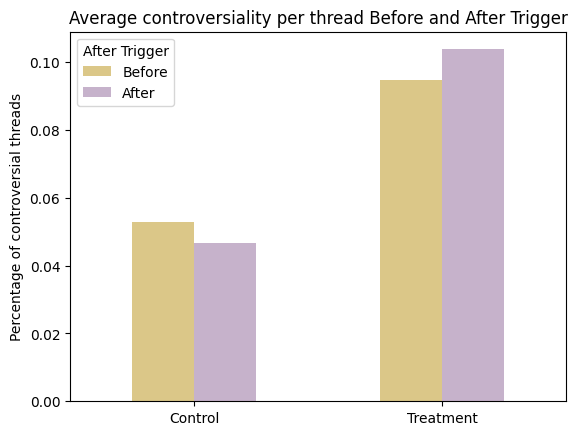
\includegraphics[width=\textwidth]{../figures/triggers/controversiality/rwanda_space.png}
    }
    \caption{Average controversiality per thread for the treatment and control (space) groups of \textit{Rwanda}.}
    \label{fig:controversiality_rwanda}
\end{figure}

\noindent\textbf{Controversiality.} We analyse the average controversiality of each thread and compare the proportion of controversial comments before and after the introduction of the trigger words. Our results (Table~\ref{tab:trigger-results}) indicate that, in general, there is an increase in controversial comments following each trigger word. Most terms display a statistically significant increase of DiD estimates when considering controversial messages in the treatment and control groups, with the biggest difference observed on the contextual comparison for \textit{Rwanda}\textemdash a causal effect of 6.6\% points. 


\begin{figure}[t!]
    \centering
    \begin{subfigure}[b]{0.7\textwidth}
        \centering
        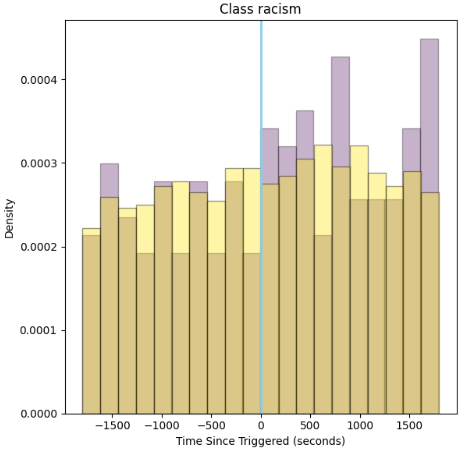
\includegraphics[width=\textwidth]{../figures/triggers/hate/space/rwanda.png}
        \caption{Rwanda}
        \label{fig:image1}
    \end{subfigure}
    \hfill
    \begin{subfigure}[b]{0.7\textwidth}
        \centering
        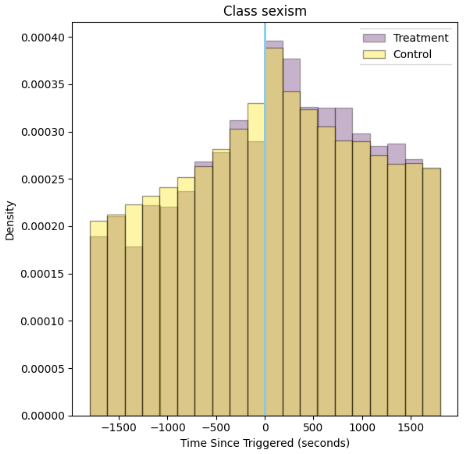
\includegraphics[width=\textwidth]{../figures/triggers/hate/space/feminism.png}
        \caption{Feminism}
        \label{fig:image2}
    \end{subfigure}
    \caption{Distribution of hateful comments in the treatment and control groups (space) of the trigger points \textit{Rwanda} and \textit{Feminism}.}
    \label{fig:hate_space}
\end{figure}

\clearpage

However, significant differences in controversiality do not appear across all settings. Notably, there seems to be no increase in controversial comments for \textit{Feminism}, and in the temporal and contextual settings for \textit{Vaccine} and \textit{NHS}, respectively.

Figure~\ref{fig:controversiality_rwanda} shows the percentages of controversial threads related to the trigger word \textit{Rwanda} for the space experiment, before and after its occurrence. The data indicates a noticeable increase in thread controversiality caused by the trigger word, reflected by a DiD estimate of 2.3\% points. The contextual and temporal control settings follow a similar trend, as documented in Appendix \ref{sec:appendix_counts}, Figure \ref{fig:rwanda_controv_temporal_semantic}.


\noindent\textbf{Sentiment \& emotion.}
We further investigate the effect trigger words have on sentiment and emotion. Based on our hypothesis, trigger words cause users to express more negatively charged emotions. In our analysis, we focus on the presence of negative sentiment and, more narrowly, the presence of anger in emotions.  

Table~\ref{tab:trigger-results} indicates a clear trend for the negatively charged comments of the treatment and control groups for each trigger word. We observe a significant increase in comments conveying a negative sentiment after the trigger word appears in 11 of the 12 settings tested, with the sole exception being the contextual comparison for \textit{NHS}. The largest effect in sentiment, with a DiD estimate of 5.5\% points, appears for the \textit{Rwanda} trigger word in the space and contextual experiments.

Let us consider the \textit{vaccine} trigger, Figure \ref{fig:sentiment_space_vaccine}, as an example. Here, we again plot the overall number of messages we observe. Both treatment and space control groups exhibit a similar pattern of negative sentiment density as time approaches the trigger word, with an increase in negative sentiment just before and after the trigger word is mentioned. % However, the treatment group shows more messages than the control group, suggesting that the trigger words affect the expression of negative sentiment.
However, the treatment group displays a noticeably higher volume of messages around the trigger term, suggesting that triggers amplify the expression of negative sentiment compared to the control condition.

Similarly to the increase in negative sentiment, trigger words systematically cause more anger. We observe a positive causal effect in all conditions, with only 3 non-significant effects. Substantively, we measure a causal effect that ranges from 1.4\% points more anger (\textit{Feminist}) to 5.5\% points (\textit{Vaccine contextual comparison}). As another example, the overall number of comments expressing anger in the \textit{Vaccine} treatment and space control groups increase significantly following the appearance of the trigger word, as shown in Figure \ref{fig:emotion_space_vaccine}, Appendix \ref{sec:appendix_counts}. This is further confirmed by the DiD estimates, which indicate a significant difference in anger-related comments in 9 out of 12 cases.

\noindent\textbf{Hate speech.}
As a final indicator of animosity, we also consider hate speech and abusive language, more specifically any kind of toxicity for \textit{Brexit}, \textit{NHS}, and \textit{Vaccine}, and the more domain-specific racism-related hate speech for \textit{Rwanda} and sexism-related hate speech for \textit{Feminism}. As seen from Table \ref{tab:trigger-results}, the impact of trigger words regarding the occurrence of hateful or offensive comments is not as prevalent as anger and negative sentiment. We observe significant effects in those areas where we can count on a domain-specific hate speech measure, i.e., in the cases of \textit{Feminism} (space and contextual comparison) and \textit{Rwanda} (space group).

We illustrate our findings in a visualization, where we consider all messages irrespective of the thread in which they are posted. We observe a distinct pattern, particularly in the context of \textit{Rwanda} and \textit{Feminism}, where the volume of hateful content increases after the trigger. Figure~\ref{fig:hate_space} reveals the prevalence of racist and sexist comments within the treatment groups when compared to their control group in the space experiment. 


\subsection{Robustness of Results}
We conduct a series of robustness checks designed to test the sensitivity of our results to assumptions and alternative specifications.

\paragraph{Testing the Parallel Trends Assumption.}
\label{sec:parallel_trends}
The DiD estimator relies on the assumption of parallel trends: without the treatment, the treated and control groups would follow the same trajectory over time. While there are no formal guarantees for the assumption to hold, there are means to argue in its favour. The first argument is a theoretical one. In neither of our experimental designs did we have reason to believe that the frequency of expressing animosity would not follow the same trend without the trigger word. Whether comparing treatment and control groups based on different Reddit fora (spaces), different words (contextual), or points in time (temporal), we suggest that without the respective trigger word, the relative difference between treatment and control group would remain the same.   

We implement event studies for each experiment to further empirically support our argument. The central idea is to model the respective outcome variable as it unfolds over time, which allows us to assess the dynamics of treatment impact before and after the intervention. Plotting the treatment effects at different time points before the treatment, the event study helps visualize whether the pre-treatment trends in the treatment and control groups are indeed parallel. If the trends are not parallel before the intervention, the parallel trends assumption is violated, indicating potential bias in the DID estimator \cite{roth2023s}. 

For each of our overall 60 experiments, we divide the 30 minutes before and after the first mention of a trigger word into six distinct time intervals $\{[-30, -20[, [-20, -10[, [-10, 0[, [0, 10[, [10, 20[, [20, 30[\}$ instead of just two. This allows us to follow, in particular, the pre-treatment trends at a higher granularity. We calculate each discussion thread's share of (hostile) messages in the six intervals. Averaging over all these data points per period, we subtract the control group from the treatment group and calculate the difference of each observation from the first observation period.

Figure~\ref{fig:robustness} charts the time-wise means over all 60 event studies. If the parallel trends assumption holds, the lines before the treatment at time = 0 should all remain on the horizontal line where the treatment effect = 0. Indeed, this is largely what we find. The mean treatment effect is close to 0 before the trigger word is mentioned for the first time. After the intervention, it is clearly above the horizontal 0-line.\footnote{See Appendix for figures that include individual event studies for all experiments from H1 and H2.}


\begin{figure}[h!]
    \centering
    \scalebox{0.9}{
    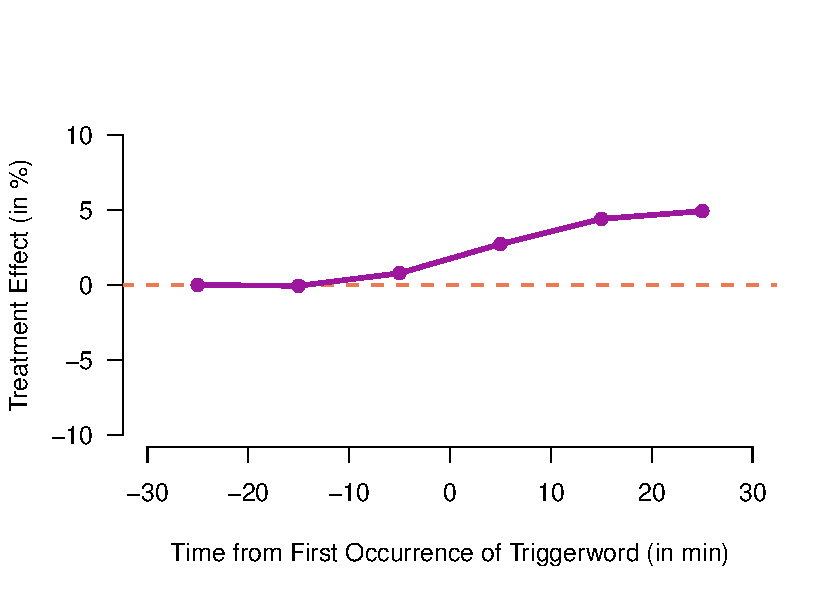
\includegraphics[width=\textwidth]{../figures/triggers/robustness_event_study.pdf}
    }
    \caption{Testing the Parallel Trends Assumption with event studies. Time-wise mean of all individual event studies in purple.}
    \label{fig:robustness}
\end{figure}

\paragraph{Placebo Treatment.}
To further validate our Difference-in-Differences (DiD) estimates, we implement a placebo treatment analysis. The core logic of this approach is to check whether the estimated treatment effects could be driven by other trends earlier or later than the actual intervention. 

In the placebo analysis, we systematically shift the assumed treatment time in 10-minute intervals, ranging from 30 minutes before to 30 minutes after the actual intervention, i.e., the comment with the first mention of the trigger word in a discussion thread. At each placebo point, we re-estimate all DiD models as if the treatment had occurred at that alternative time. If our results capture a genuine causal effect, we expect a pronounced treatment effect at the actual intervention time ($t = 0$), and near-zero or statistically insignificant estimates at all placebo points before and after.

\begin{figure}[h!]
    \centering
    \scalebox{0.9}{
    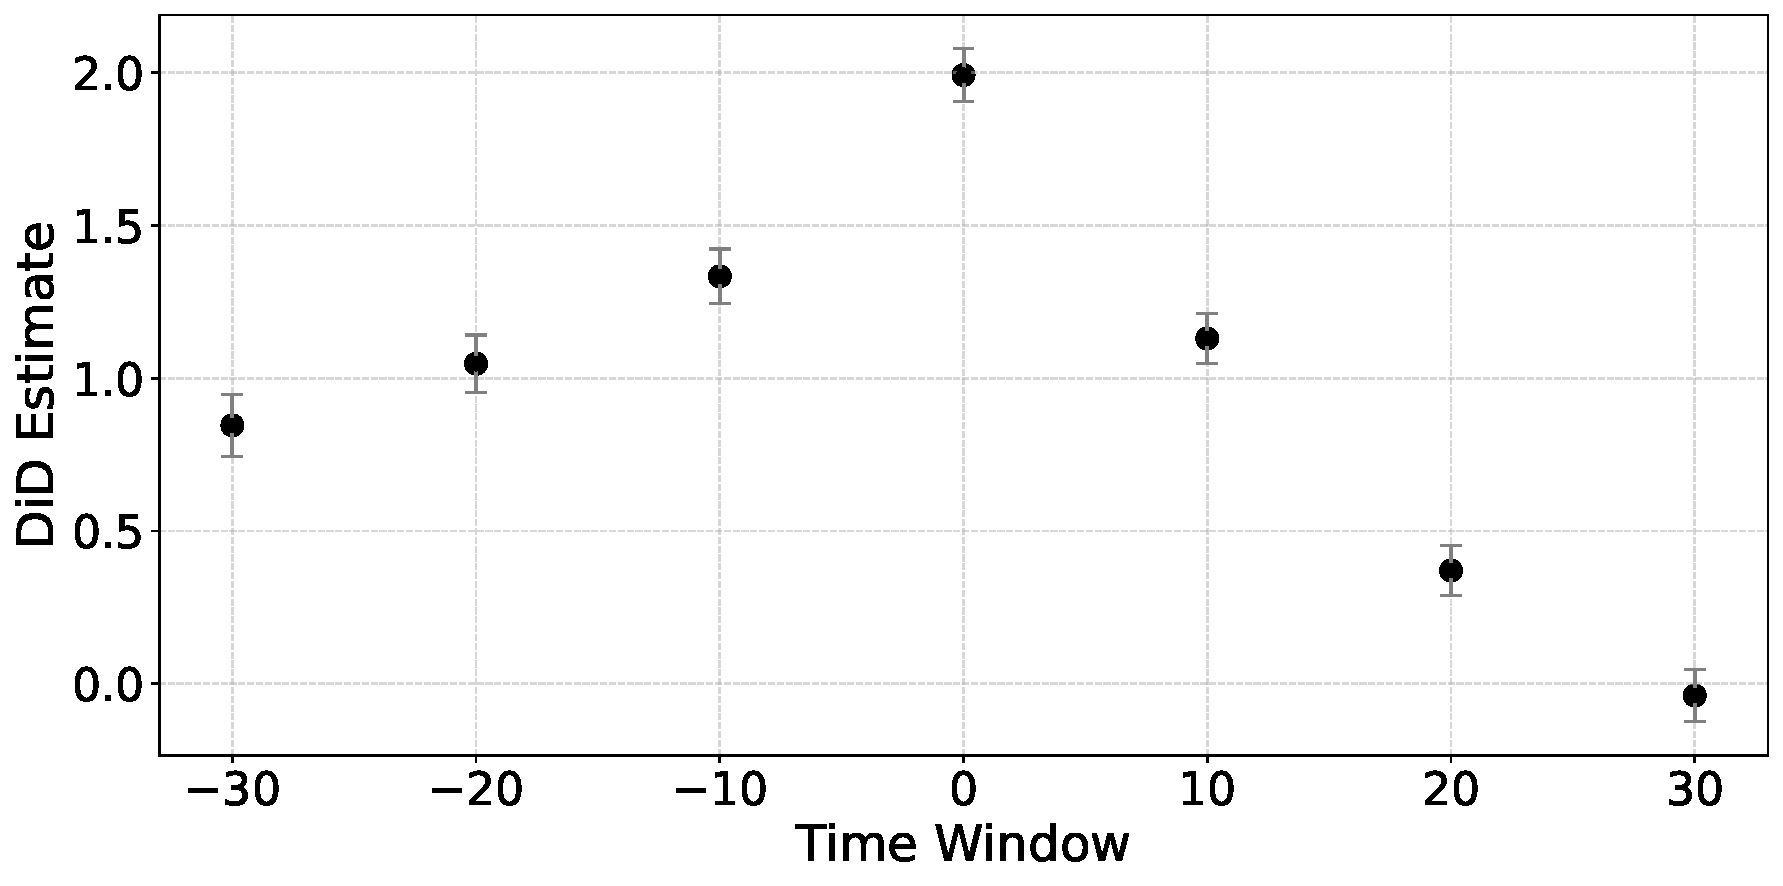
\includegraphics[width=\textwidth]{../figures/triggers/placebos.pdf}
    }
    \caption{Placebo treatments every 10 minutes, ranging from 30 minutes before to 30 minutes after the actual treatment point. Precision weighted average treatment effects and 95\% confidence intervals across all experiments.}
    \label{fig:placebos}
\end{figure}

Figure~\ref{fig:placebos} visualizes these placebo tests by plotting the precision-weighted average treatment effects and their confidence intervals across all experiments measuring animosity (see Table~\ref{tab:trigger-results}). At the actual treatment point $t = 0$, which compares message content in the 30 minutes before and after the first appearance of the trigger word ($[-30,0[$ vs. $[0,30]$), we observe a clear and substantial effect (1.99). We then shift the treatment window rightward in 10-minute steps—first comparing $[-20,10[$ to $[10,40]$, and so on—until the actual intervention fully exits the analysis window at $t = 30$. This generates a steady decline in estimated effects, which converge to zero, as expected if no real treatment occurred at these placebo times. Similarly, shifting the window to earlier times (e.g., comparing $[-60,-30[$ to $[-30,0]$) reveals a decreasing trend in effect size, though some residual difference remains. In conclusion, given the clear peak of the effect at the timing $t=0$, we are confident in the robustness of our approach to defining the moment of the actual treatment moment.



\section{Conclusion}
% If we found no evidence for the theory, we could refute the theory early on. However, given we indeed find evidence for it, we suggest 
This chapter establishes trigger words as a concept in online debates. Since our work represents the first systematic computational study of this concept, our research design and case selection are geared to clearly identify such behaviour in the most likely cases. To do so, we performed a large-scale analysis about UK politics on Reddit using five trigger words (\textit{Rwanda, Feminism, Brexit, NHS, and Vaccine}). 

The results show that trigger words cause more user engagement, and this activity is marked by higher levels of animosity. This confirms the first hypothesis (H1), which suggests more user interaction after the appearance of a trigger word. Regarding our second hypothesis (H2), which concerns the impact of trigger words on the animosity of the ensuing discussions, we examine four different features that can indicate such effects. Trigger words cause more controversiality, more negative sentiment, and more anger. We also investigate the causal effect of trigger words on hate speech. Where we can, we rely on a model capable of identifying domain-specific forms of hate \textemdash sexism in the case of \textit{Feminism} and racism in the case of \textit{Rwanda}\textemdash. Our findings similarly confirm that trigger words play a causal role in this aspect as well.

From this work, we can certify that trigger points exist in online communication, and we have provided a framework to measure the extent of them in terms of user engagement and animosity. Future work will analyse this phenomenon more comprehensively. We aim to broaden the scope, study how prevalent trigger points are in different countries and languages, and seek to better understand further behavioural consequences from trigger points. It is our intention to evaluate the extent to which trigger points are responsible for hateful online communication. We also strive to automate the trigger point detection process to detect the respective words in online conversations when we do not know them \emph{ex-ante}.

\section{Limitations}
We refrain from using large language models (LLMs) for feature extraction mainly due to the vast size of our dataset ($>$100 million entries). Using LLMs would have significantly increased the computational and financial cost and the ecological impact of our experiments. Moreover, existing literature indicates that the zero-shot capabilities of LLMs do not consistently outperform smaller models for specific social media tasks like ours \cite{antypas-etal-2023-supertweeteval}.

Our study does not attempt to map how pervasive trigger points are in online debates. The chosen subreddits may not fully represent the broader range of discussions these trigger words could provoke across the diverse Reddit community. Similarly, we acknowledge the limitations and potential biases of our work, as we only investigate a small set of potential trigger words in the context of the UK and limit our data to comments written in English in a limited selection of subreddits. The choice of trigger words is informed by a contextual analysis of the UK politics, and the Reddit threads have been selected due to the often polarised conversations they host around such topics. However, this is the first study that analyses trigger points' concept validity in online conversations. Based on our empirical evidence, we can be confident that we have found relevant evidence that warrants further investigation. 

\section{Ethics Statement}
All data used in our research is sourced from publicly available information or collected using the official Reddit API. It is provided in an aggregated way and without reporting sensitive information from individual users.

The automatic methods used can be abused by those with the power to repress people with opposing opinions. Hence, we offer a comprehensive study but do not share our data publicly to avoid potential misuse or commercial use. Researchers interested in replicating our experiments can contact us directly.
